\chapter{Implementación}


\section{Controladores}

El controlador digital presentado en la sección \ref{cap3_controladores} se implementó en lenguaje C usando la transformada directa II.

%https://www.keil.com/pack/doc/CMSIS/DSP/html/group__BiquadCascadeDF2T.html


\subsection{Microcontrolador}



\subsection{Puente H}

Funciones especificas

\section{Integración de hardware}

Esquematico y componentes

\subsubsection{PCB}

Placa PCB

\section{Bus de campo}

Conexión


\section{Software}

\subsection{ROS}

Como se monstró en el capitulo pasado, su utilizó ROS como framework para realizar la integración. Los dispositivos de hardware, el robot Scorbot y el dispotivo háptico Phantom, cuentan con su \textit{nodo driver} que permiten la integración con el ecosistema ROS.

Se entiende por \textit{nodo driver} o ROS \textit{wrapper}, a una aplicación que actua como puente entre un dispositivo fisico y su representación en ROS, permitiendo interactuar de forma transparente con el dispositivo mediante el uso tópicos y servicios. Usualmente el \textit{nodo driver} hace uso de librerías proveidas por el fabricante o terceros para el manejo protocolos especificos del dispositivo. Por ejemplo, las siguientes aplicaciones cumplen esta función:

\begin{itemize}

\item \textit{ROSARIA}\cite{rosaria}: corresponde a una aplicación construido usando la librería \textit{Adept MobileRobots Robotics Interface for Applications} (ARIA), permite el control de robots móviles de las compañias Adept MobileRobots, MobileRobots Inc., y ActivMedia, por ejemplo el Pioneer 3-DX y 3-AT.

\item \textit{kinova-ros}\cite{kinova}: Es el driver oficial ofrecido por Kinova robotics para el uso de los robot manipuladores Jaco y Mico.

\end{itemize}

\subsubsection{Integración del robot Scorbot}

En esta sección se describirá la función de cada uno de los nodos que integran el software desarrollado para el control del robot Scorbot.

\begin{figure}[ht]
  \centering
  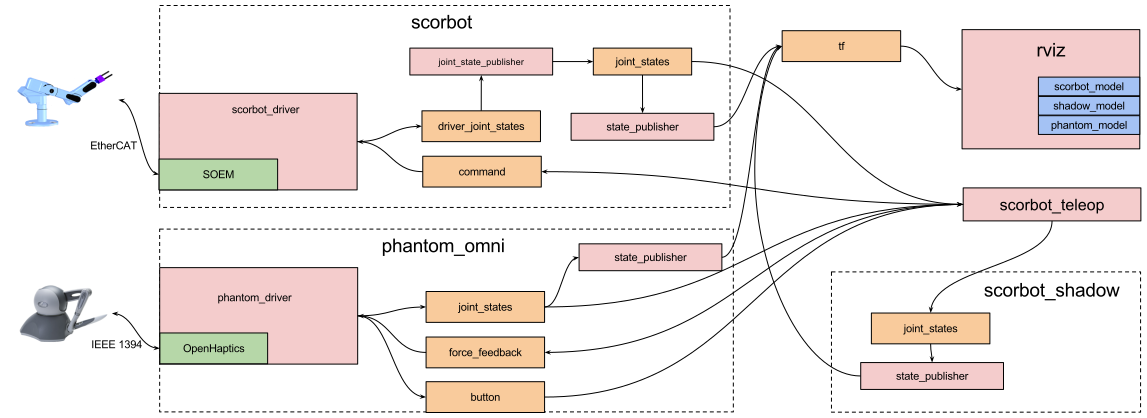
\includegraphics[width=\textwidth]{img/cap4/scorbot_software.pdf}
  \caption{Diagrama de nodos y tópicos de la aplicación.}
  \label{cap4_scorbot_software}
\end{figure}

\begin{description}

\item[\texttt{scorbot\_driver}] Corresponde al \textit{nodo driver} se integra con la librería SOEM \cite{soem} para la comunicación EtherCAT. Dado que este nodo ejecuta un ciclo de control, se consideraron una serie de requerimientos, muchos de ellos básicos para software de ejecución en tiempo real:

\begin{itemize}
\item Separación de hilos de ejecución, todas las tareas realacionadas con actualización de datos en el bus de control se realiza en un hilo independiente (\textit{control thread}) a las comunicaciones con el framework ROS (ROS \textit{thread}).
\item La comunicación entre el  \textit{control thread} y el ROS \textit{thread} se realiza usando estructuras de datos no bloqueantes.
\item La memoria utilizada por el hilo de control queda fija luego de la inicialización, de esta forma no se hacen llamados al sistema para pedir o liberar memoria.
\end{itemize}

SOEM mapea en memoria los dispositivos, es decir, desde el la aplicación master se tiene acceso a un buffer de memoria que permite leer y escribir en los dispositivos esclavos. Para obtener los datos manipulables, se debe usar la misma estructura de datos que usa el dispositivo esclavo para representar la información. \texttt{setpoint\_t} es la estructura usada como referenca (\textit{set point}), miestras que \texttt{joint\_data\_t} es la información del estado del controlador. Estas estructuras estan contenidas en un archivo de cabezera generado por el SSC, su modificación debe realizarse de forma cuidadosa, pues se pueden obtener errores de representación.

\begin{lstlisting}[language=C, caption=Estructuras de datos usadas para mapear datos de dispositivos esclavos]
typedef struct PACKED {
    uint16_t controlRegA;
    uint16_t controlRegB;
    int16_t  currentRef;
    int16_t currentLim;
    uint16_t pidCurrentKp;
    uint16_t pidCurrentKi;
    uint16_t pidCurrentKd;
} setpoint_t;

typedef struct PACKED {
    int16_t encPosition;
    int16_t encSpeed;
    int16_t current;
    uint16_t limits;
} joint_data_t;
\end{lstlisting}

\begin{figure}[ht]
  \centering
  \includegraphics[width=\textwidth]{img/cap4/scorbot_driver.pdf}
  \caption{Diagrama del nodo \texttt{scorbot\_driver}.}
  \label{cap4_scorbot_driver}
\end{figure}

\end{description}




